\documentclass{article}
\usepackage{float}
\usepackage{comment}
\usepackage{arxiv}
\usepackage[utf8]{inputenc} % allow utf-8 input
\usepackage[T1]{fontenc}    % use 8-bit T1 fonts
\usepackage{hyperref}       % hyperlinks
\usepackage{url}            % simple URL typesetting
\usepackage{booktabs}       % professional-quality tables
\usepackage{amsfonts}       % blackboard math symbols
\usepackage{nicefrac}       % compact symbols for 1/2, etc.
\usepackage{microtype}      % microtypography
\usepackage{lipsum}
\usepackage{graphicx}
\usepackage{braket}
\graphicspath{ {./images/} }
\usepackage[english]{babel}
\usepackage[square,numbers]{natbib}
\bibliographystyle{unsrt}
\usepackage{amssymb}
\NewDocumentCommand{\tens}{t_}
 {%
  \IfBooleanTF{#1}
   {\tensop}
   {\otimes}%
 }

\title{Classification via Quantum Machine Learning} %or 
%Quantum Machine Learning for Classification
% Enhancing Classification Algorithms with Quantum Machine Learning
% Classification via Quantum Machine Learning

\author{
 Sánchez Rolando \\
 School of Physical Sciences and Nanotechnology\\
 Yachay Tech University\\
 Urcuquí - Ecuador. \\
 \texttt{rolando.sanchez@yachaytech.edu.ec} \\
 \And
 Mowbray Duncan \\
 School of Physical Sciences and Nanotechnology\\
 Yachay Tech University\\
 Urcuquí - Ecuador. \\
 \texttt{	duncan.mowbray@yachaytech.edu.ec} \\
}


\begin{document}
\maketitle
\begin{abstract}
Classification is a key component of various scientific, technological and industrial domains, from biomedical diagnostics and computational materials science to finance, climate modeling, and sociology. However, classical machine learning (ML) approaches often face limitations in computational efficiency, especially for high-dimensional and complex datasets, where quantum computing has been proposed as a promising breakthrough. Quantum machine learning (QML) has recently attracted much interest, intending to leverage the potential of quantum computing to achieve computational advantages over classical methods. Notable quantum algorithms, such as the Harrow-Hassidim-Lloyd (HHL) solver for linear systems and Shor's algorithm for integer factorization, demonstrate exponential speedups for specific tasks, suggesting the potential of quantum computing to revolutionize the computational landscape. In this mini-review, we explore the current state of the art of quantum classification algorithms, focusing on quantum support vector machines (QSVM), their implementations using the Qiskit software framework and their performance. By critically evaluating their advantages and limitations, we evaluate whether QML represents a transformative paradigm or remains constrained by challenges in hardware, scalability, and decoherence. Finally, we will highlight the role of hybrid classical-quantum approaches and the advancements needed to realize quantum-enhanced classification in practical applications.
\end{abstract}

% keywords can be removed
%\keywords{Machine Learning \and Quantum Mechanics \and Quantum Machine Learning \and Classification} 

\section*{Introduction}

Classification is probably the most essential component of any activity, regardless of whether it is for scientific purposes. Its wide-ranging applications include finance, climate modelling, biomedical diagnostics, computational materials science, sociology, and human behaviour. Data is categorized into distinct groups to generate precise predictive models through classification. Typically, these issues are grouped into two primary categories: binary classification and multi-class classification. The binary classification process entails dividing data into two categories, such as identifying spam versus non-spam emails or differentiating between cancerous and non-cancerous tissues in medical diagnosis.
In contrast, multi-classification encompasses additional categories, such as identifying skin lesion types associated with cancerous conditions \cite{10613907skin}. On the other hand, computational resources frequently present substantial obstacles to implementing ML approaches. These constraints have sparked interest in investigating alternative computational paradigms, with quantum computing emerging as a promising candidate to address these bottlenecks.

ML is a branch of computer science focused on identifying patterns in data attributes to make predictions about previously unseen inputs. It involves creating algorithms that enable computers to learn from data and make decisions autonomously, without being explicitly programmed for specific tasks. These algorithms are generally categorized into three main types: supervised, unsupervised, and reinforcement learning \cite{Ayodele10}.

Supervised learning relies on a labeled training dataset, where input-output relationships are clearly defined, allowing the algorithm to learn and classify new data based on these examples. Unsupervised learning, on the other hand, aims to uncover hidden structures, clusters, or groupings within unlabeled data \cite{10047618}. In both cases, the core task is pattern classification, which involves assigning new input data to predefined categories or classes.

Reinforcement learning, which mimics aspects of human learning, operates within a framework of rules and objectives. Here, the algorithm receives rewards or penalties based on the actions it takes to achieve a goal. Rewards reinforce successful strategies, while penalties prompt adjustments to improve decision-making. While reinforcement learning is a powerful approach, this work will not focus on it, as the primary application under review is classification.

A significant challenge in ML is the computational time and storage required, especially when dealing with large datasets. Additionally, training these models is time-intensive as the main challenges lie in the problem of finding the right parameters that lead to an optimal solution. To address these limitations, researchers have turned to quantum computing as a promising alternative. Quantum methods have the potential to significantly reduce both storage requirements and computational time, offering a new direction for overcoming the constraints of classical approaches \cite{degruyterIntroductionQuantum}.

The most noticeable advantage of quantum computing is the ability of manipulate quantum states in superposition in order to speed up computational tasks in terms of complexity, as these operations would be executed on many states at the same time. In a formal way, quantum computers surpass classical ones by using qubits, which exist in an exponentially larger space, $\mathbb{SU}(2^n)$, compared to classical bits in Boolean space, $\mathbb{B}^{\tens{} n} $. While an n-bit classical register holds one n-digit binary string, a quantum register of the same size can represent all possible strings simultaneously, offering an exponential advantage \cite{Nielsen_Chuang_2010}. Then, quantum algorithms are developed such that the modified quantum state has a high amplitude for states representing solutions for a given problem. 
However, while quantum supremacy has been demonstrated for specific problems \cite{Arute2019}, achieving it in data science remains uncertain, even theoretically. Nonetheless, this is a key objective in QML.

Usually, QML is considered for four main tasks as shown in Fig.\ref{fig:qtasks}, where CC tasks refers to classical computers using quantum computing inspired algorithms to process classical data, such as recommendation system algorithms \cite{ccalg}. CQ refers to processing classical data using QML algorithms \cite{cq}. QC setting asks how classical learning techniques may
help in quantum tasks and this is an active area of investigation, with classical machine learning algorithms used in many areas in the quantum computing, such as qubit characterization \cite{charqc}, control \cite{controlqc} and readout\cite{readoutqc}. Finally, QQ, a field remaining in its early stages, involves the processing of quantum data with quantum machine learning algorithms, for instance, analyzing molecular ground state energy directly in quantum computers using QML to optimize processes.
\begin{figure}[h!]
    \centering
    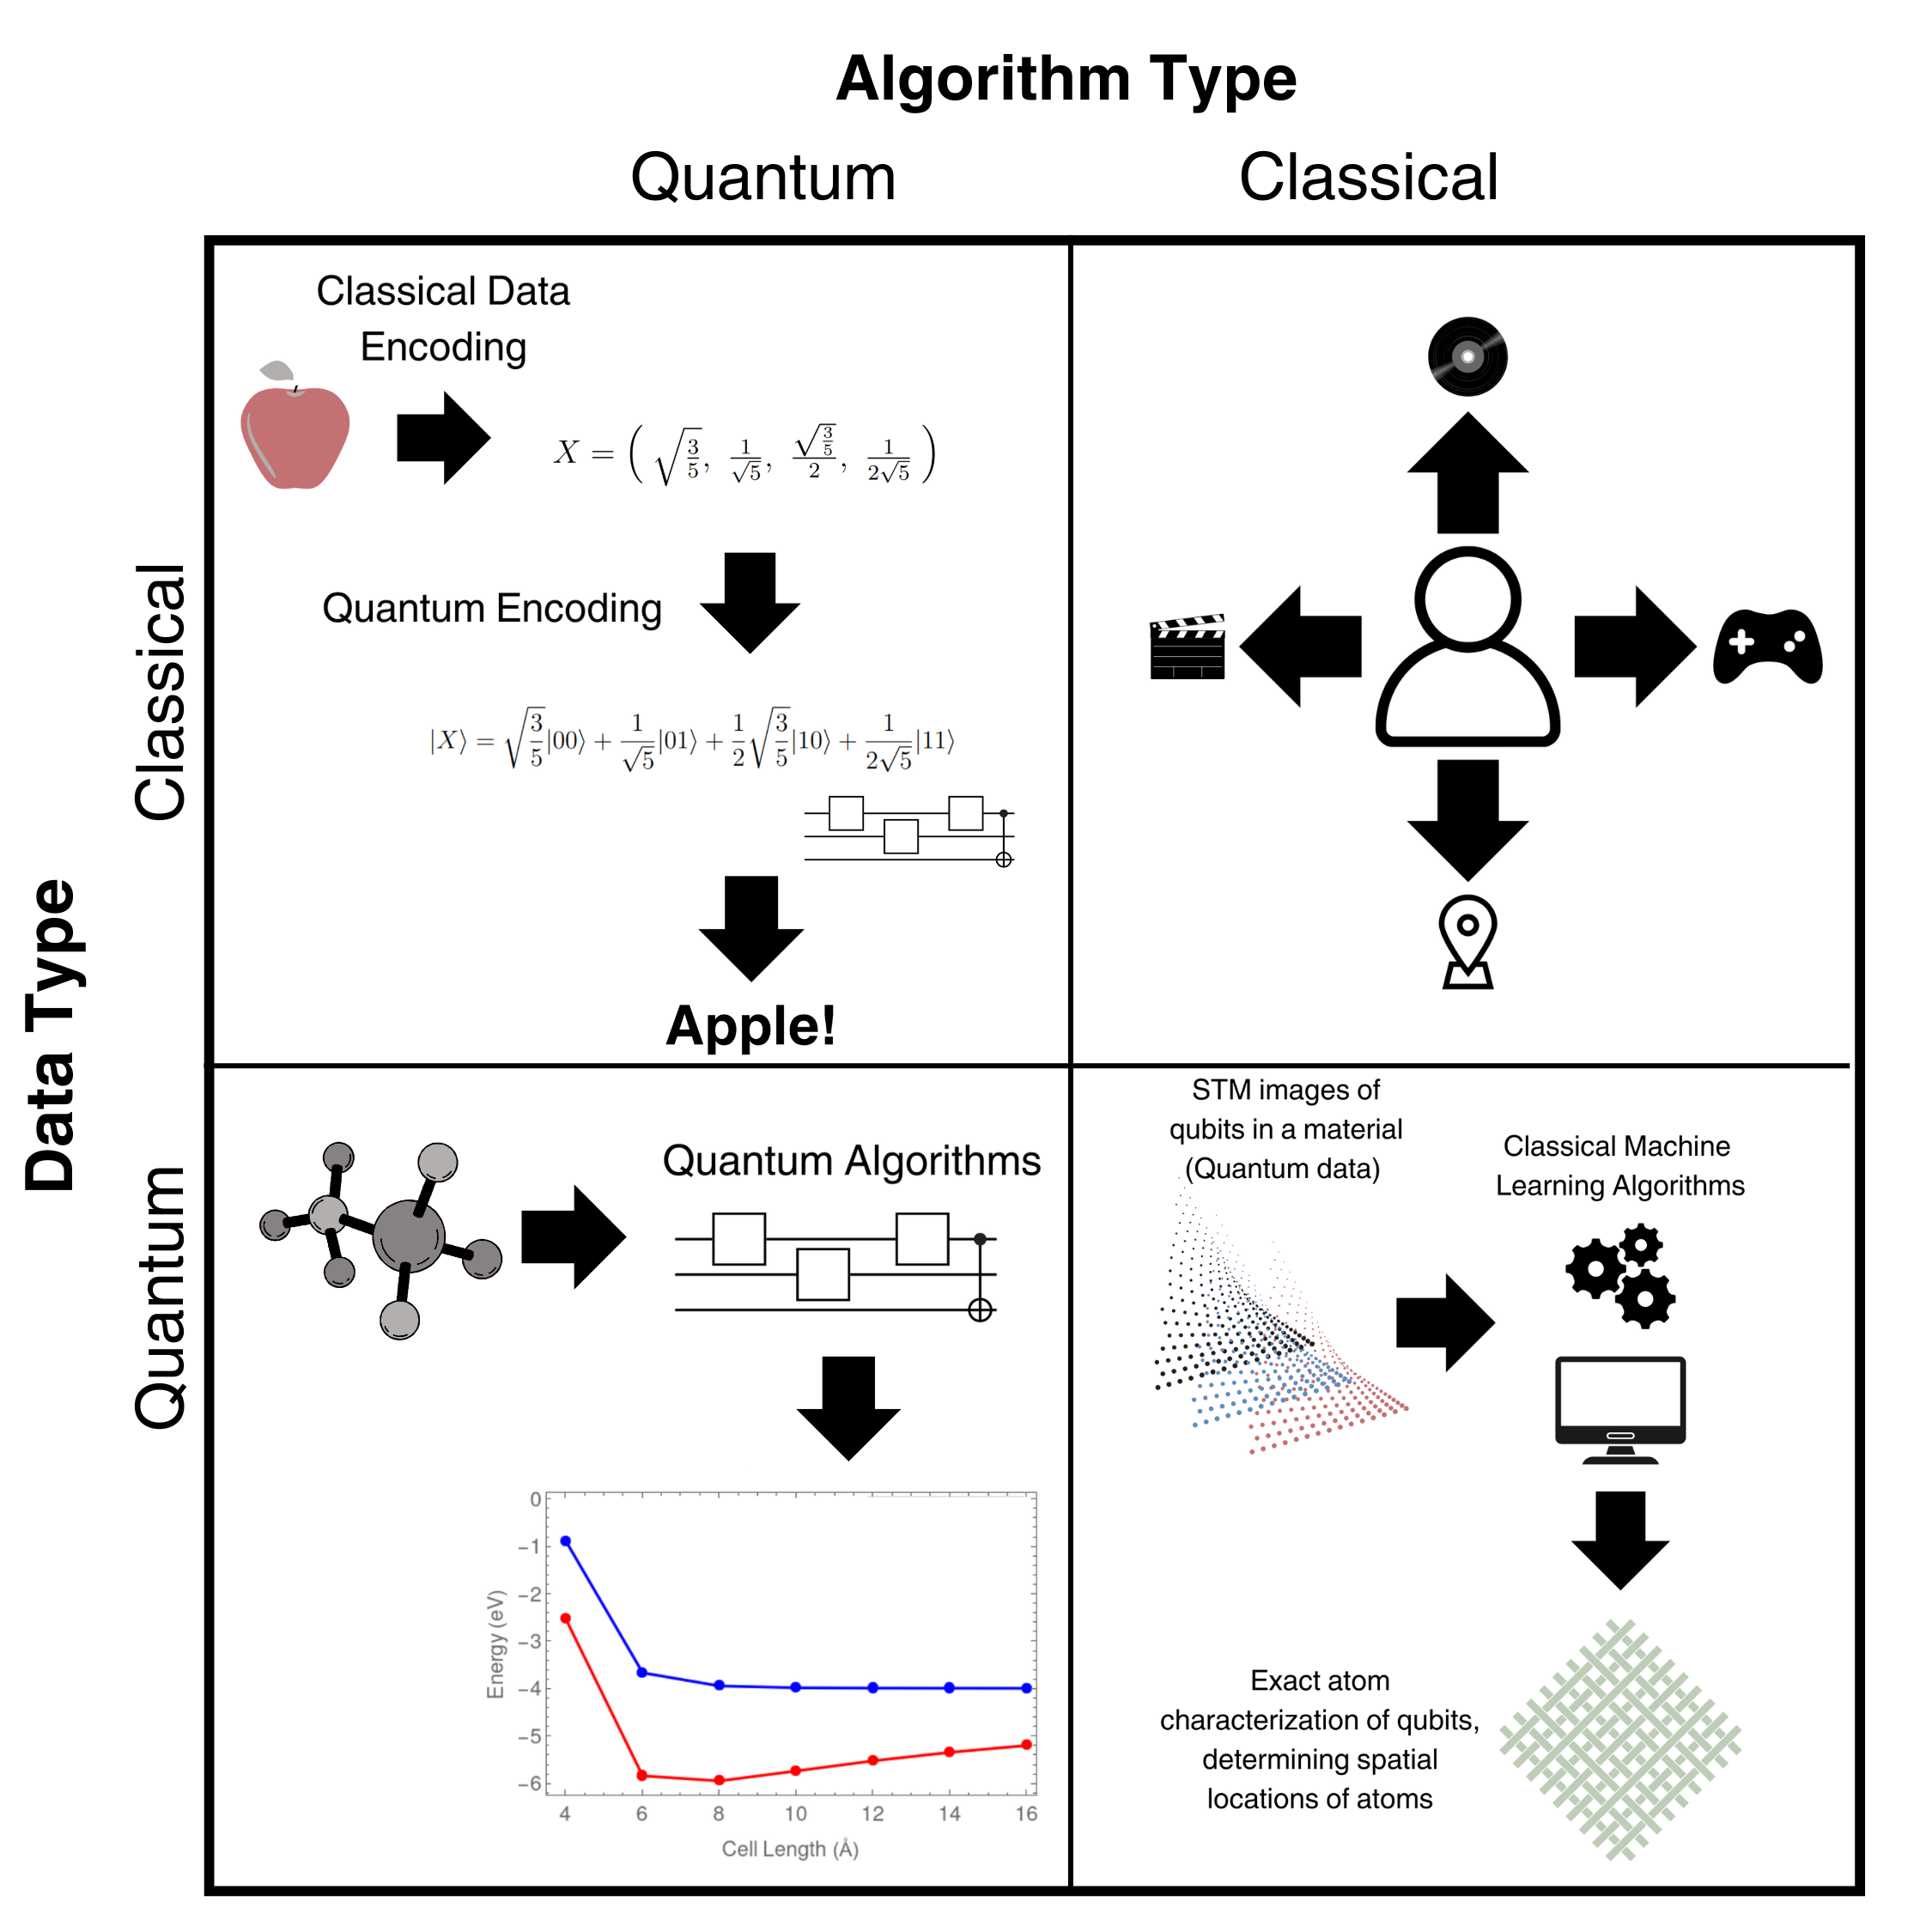
\includegraphics[scale=0.19]{figures/QMLtypes.png}
    \caption{QML four main tasks}
    \label{fig:qtasks}
\end{figure}

In this article, we provide a comprehensive review of the current state of quantum classification algorithms, specifically emphasizing the implementation of QSVMs. We critically assess the potential of these algorithms to revolutionize classification tasks in practical applications by evaluating their advantages and limitations. This work aims to determine whether QML is a transformative paradigm or if existing technological challenges still constrain it by analyzing the interaction between quantum computing and machine learning.


\section*{Quantum Classification Algorithms}
\subsection*{Quantum k-nearest neighbours}
The classical k-nearest neighbours algorithm assigns a class to an unclassified object by comparing its vector $\vec{v}$ to previously classified training samples. This is done using a distance metric, typically Euclidean or Hamming distance, to identify the k-nearest neighbours in the multidimensional space. The steps of the algorithm can be summarized as follows:

\begin{enumerate}
    \item Choose a distance metric and compute the distance between the unclassified object vector $\vec{v}$ and each training sample.
    \item Identify the $k$ training samples closest to $\vec{v}$ based on the chosen metric.
    \item Assign the class with the highest frequency among the $k$ nearest samples to the object $\vec{v}$.
\end{enumerate}

This approach relies on the assumption that objects close to each other in the multidimensional space share similar properties. Translating this concept into a quantum framework requires redefining distance metrics in quantum terms. Building on the data representation proposed by Lloyd et al. \cite{Lloyd2013}, as shown in Eq. \ref{eq:1}, a method was developed to quantify the distance between classical object vectors $\vec{x}$ and $\vec{y}$ using quantum measurements.

\begin{equation}
    \ket{v} = |v|^{-\frac{1}{2}} \vec{v}
    \label{eq:1}
\end{equation}

The authors begin by calculating the inner product of the ancilla state $\ket{\psi} = \frac{\sqrt{2}}{2} (\ket{0, x} + \ket{1,y})$ with the state $\ket{\phi} = \frac{\sqrt{Z}}{Z}(|\vec{x}|\ket{0} - |\vec{y}|\ket{1})$, where $Z = |\vec{x}|^2 + |\vec{y}|^2$ ensures normalization. This leads to the identity in Eq. \ref{eq:2}, which provides a way to compute the distance between the vectors.

\begin{equation}
    |\vec{x} - \vec{y}|^2 = Z \, |\braket{\psi | \phi}|^2
    \label{eq:2}
\end{equation}

The overlap $|\braket{\psi | \phi}|^2$ in Eq. \ref{eq:2} can be physically retrieved using a routine known as the swap test \cite{swaptest}. The probability of measuring the initial state $\ket{\xi}$ in this test is given by Eq. \ref{eq:3}, where the overlap appears explicitly.

\begin{equation}
    P(\ket{\xi}) = \frac{1 + |\braket{\psi | \phi}|^2}{2}
    \label{eq:3}
\end{equation}

Using these principles, a quantum version of the nearest centroid algorithm can be constructed. Here, $\vec{x}$ represents the sample to be classified, and $\vec{y} = \frac{\sum_p \vec{v}^p}{N_c}$ is the centroid of a given class. The authors argue that this quantum method, including the construction of quantum states, achieves greater efficiency than the classical polynomial runtime.

\subsection*{Quantum Neural Networks (QNNs)}
Classical neural networks (NNs) are computational models inspired by biological neurons, processing input data through layered architectures of interconnected nodes to produce a desired classification output. As illustrated in Fig. \ref{fig:qnn1}, these models adjust their parameters via backpropagation to minimize a predefined loss function, optimizing their predictive performance through iterative training. On the other hand, QNNs are a specialized subclass of variational quantum algorithms, implemented using parameterized quantum circuits. These circuits employ tunable unitary rotation gates and entangling operations to perform numerical tasks such as optimization, approximation, and classification \cite{kwak2021quantumneuralnetworksconcepts}.

The operational workflow of a common QNN involves the stages shown in Fig. \ref{fig:qnn1}. First, classical input data is encoded into a quantum state using a feature map \cite{kwon2024featuremapquantumdata}, initializing the qubit register. Next, a variational circuit transforms this initial encoded quantum state across multiple layers. The final quantum state is then measured by evaluating the expectation value of a Hamiltonian operator, typically represented by Pauli gates \cite{farhi2018classificationquantumneuralnetworks}. These quantum measurements are decoded into classical outputs, which are used to compute the loss function. The variational parameters are optimized to minimize this loss, analogous to classical training but within a quantum computational framework. This hybrid structure positions QNNs at the intersection of classical deep learning and parameterized quantum circuits, offering potential advantages in certain machine learning tasks while remaining subject to ongoing research and design refinements. \cite{qiskittheory}.

\begin{figure}[h!]
    \centering
    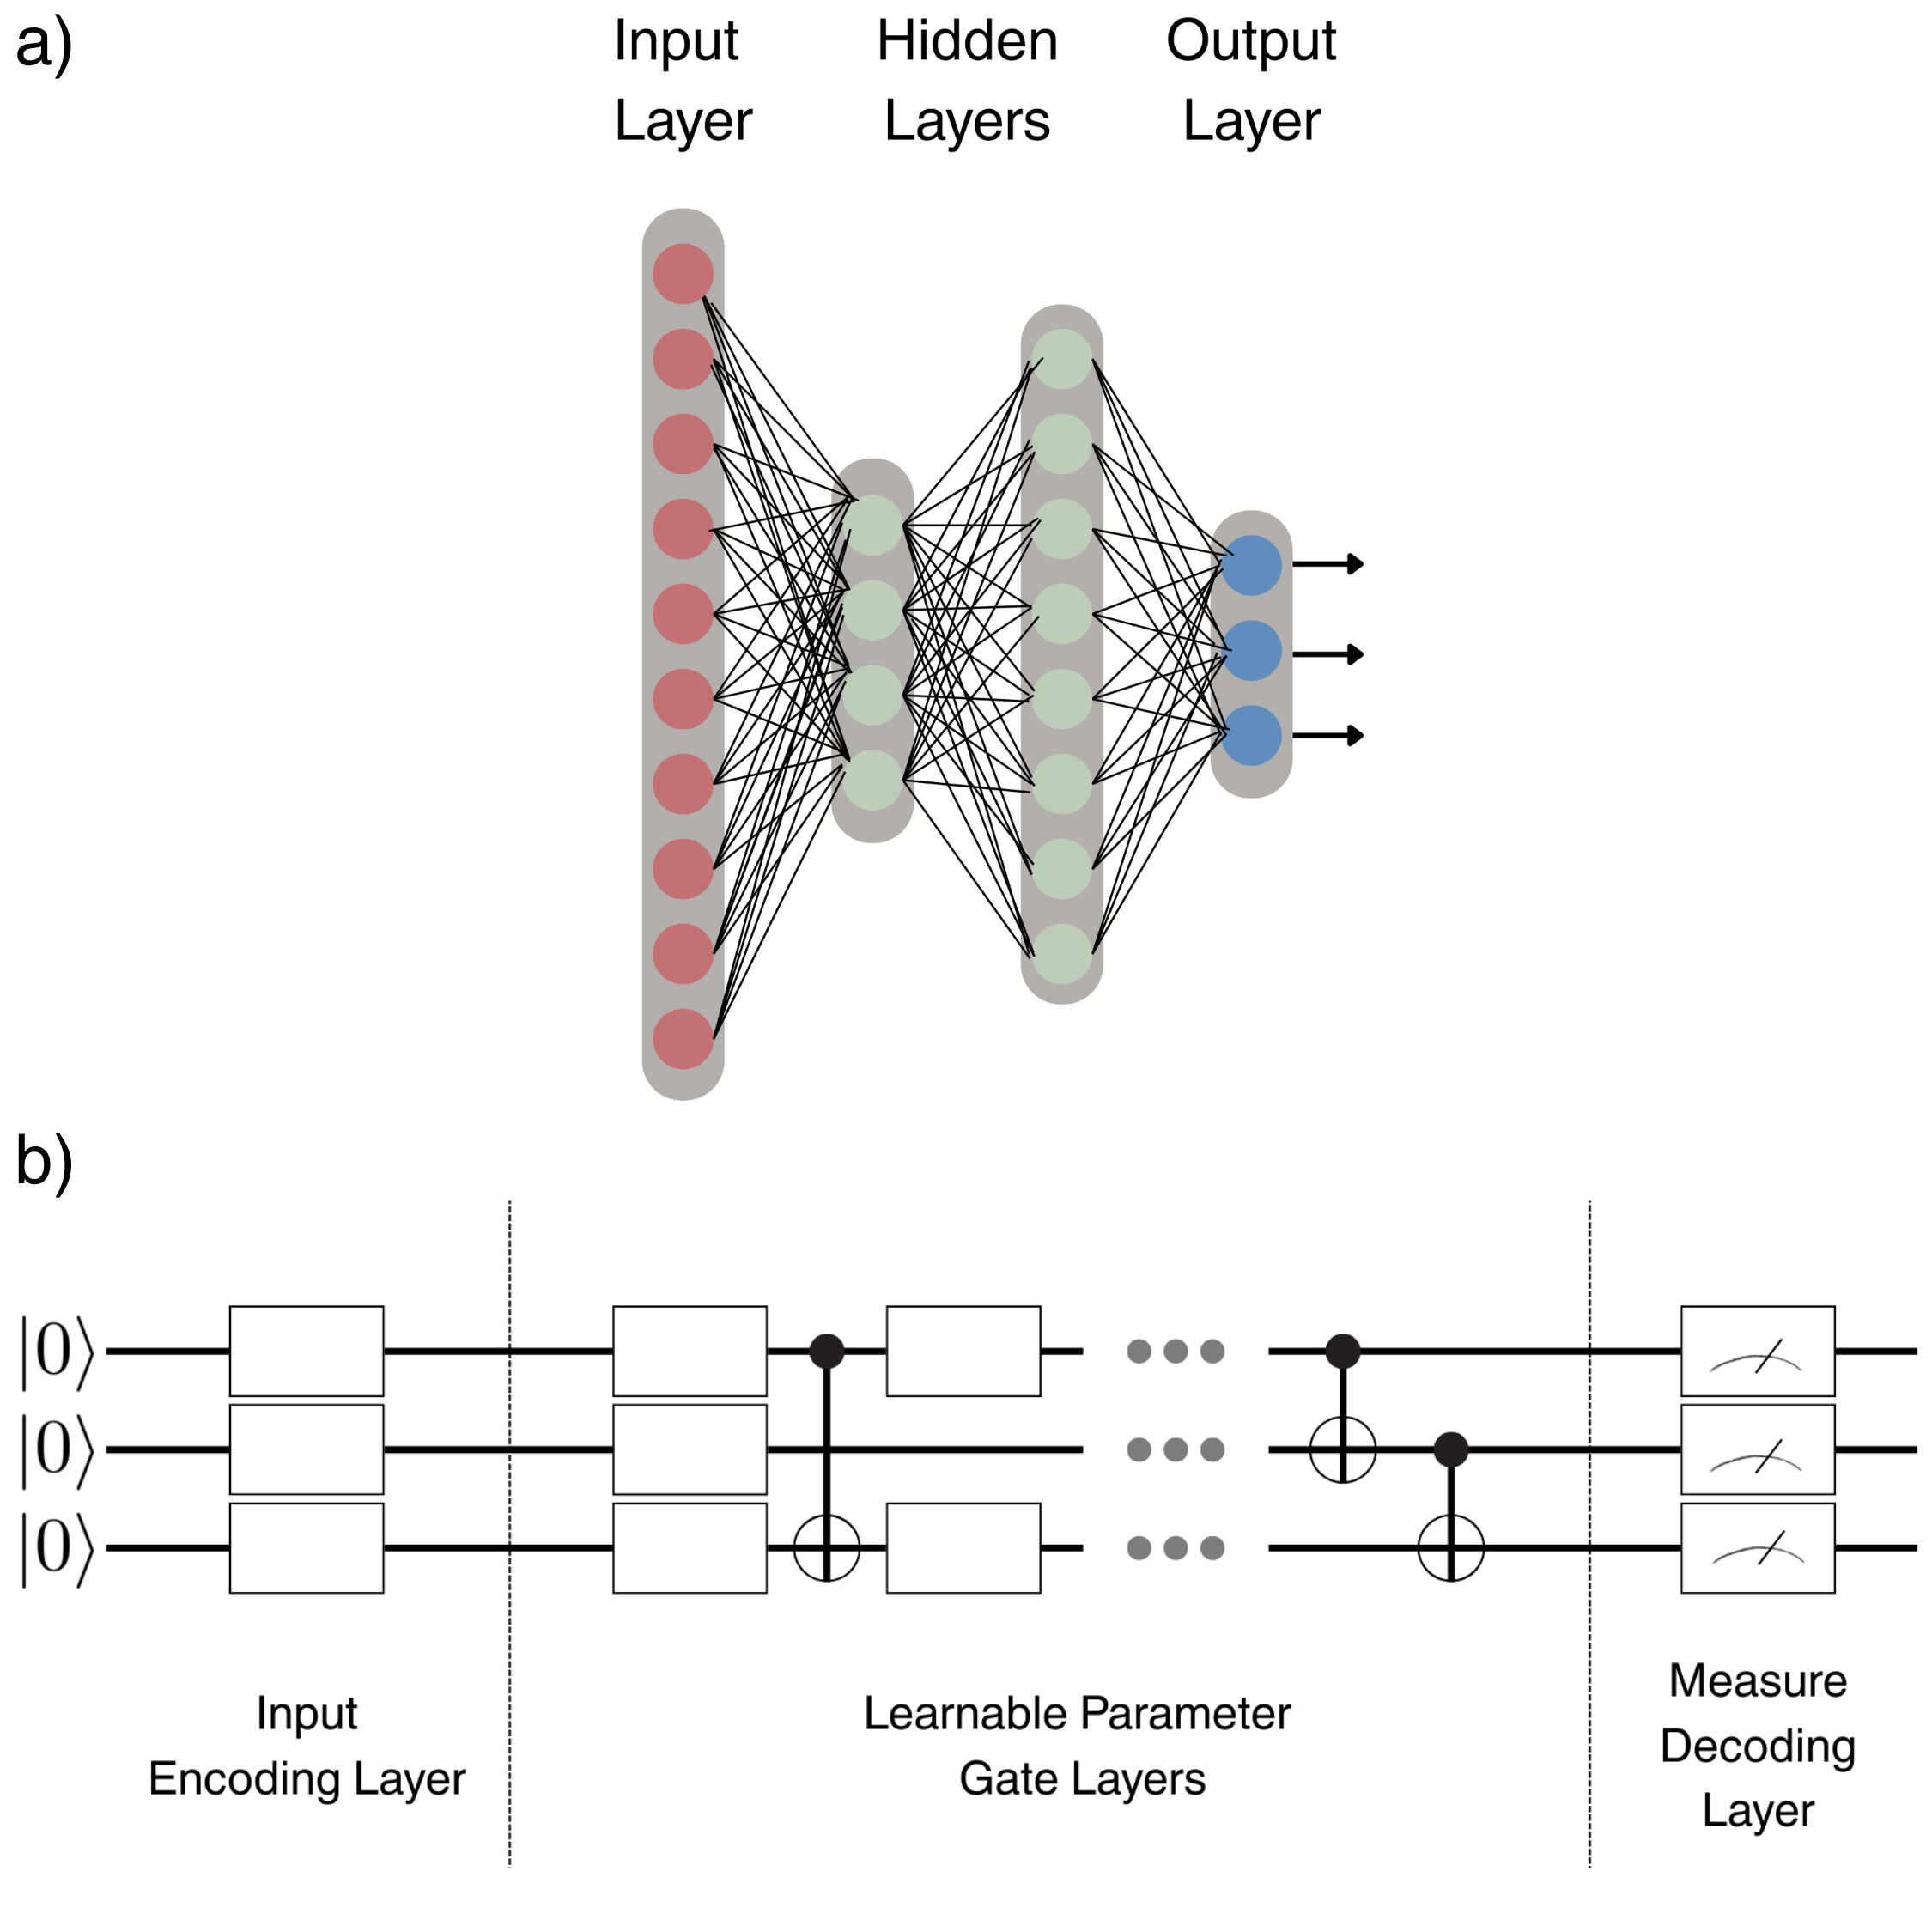
\includegraphics[scale=0.15]{figures/nns.png}
    \caption{a) Main components of classical neural networks. b) Components in proposed QNN}
    \label{fig:qnn1}
\end{figure}


Now, the previously described QNN structure is usually modified to match the specific needs of the problem. 
For instance, the feature map can be done in different ways like basis encoding, amplitude encoding, product encoding, angle encoding, etc. 
In a similar way, the variational quantum algorithm will be designed according to the problem and there are several ways to do it \cite{9528698}.
It has been demonstrated that Quantum Neural Networks (QNNs), implemented as variational quantum circuits with classical optimizers
for tuning the parameters, can outperform NNs on relatively small datasets, despite their significantly 
lower complexity and fewer parameters \cite{10015720}. For instance, QNNs achieved an average accuracy improvement of 7\% over 
classical NNs in experiments, even with orders of magnitude fewer parameters.
These advantages were also noticed in medical image classification \cite{10613907, 9293291}. 
However, these advantages were observed under the constraints of current noisy intermediate-scale quantum (NISQ) hardware, which limits problem
sizes due to qubit counts and error rates. As quantum hardware advances, it is expected that QNNs will scale to larger problem sizes, though 
challenges such as error mitigation, circuit depth limitations, and optimal entanglement strategies must first be addressed.


\subsection*{Quantum Decision Trees (QDTs)}




\begin{comment}
\paragraph{Construct train and test data.}
In the Sales train dataset, it only provides the sale within one day, but we need to predict the sale of next month. So we sum the day's sale into month's sale group by item, shop, date(within a month).
In the Sales train dataset, it only contains two columns(item id and shop id). Because we need to provide the sales of next month, we add a date column for it, which stand for the date information of next month.]

\subsection{Headings: second level}
\lipsum[5]
\begin{equation}
\xi _{ij}(t)=P(x_{t}=i,x_{t+1}=j|y,v,w;\theta)= {\frac {\alpha _{i}(t)a^{w_t}_{ij}\beta _{j}(t+1)b^{v_{t+1}}_{j}(y_{t+1})}{\sum _{i=1}^{N} \sum _{j=1}^{N} \alpha _{i}(t)a^{w_t}_{ij}\beta _{j}(t+1)b^{v_{t+1}}_{j}(y_{t+1})}}
\end{equation}

\subsubsection{Headings: third level}
\lipsum[6]

\paragraph{Paragraph}
\lipsum[7]

\section{Examples of citations, figures, tables, references}
\label{sec:others}
\lipsum[8] \cite{kour2014real,kour2014fast} and see \cite{hadash2018estimate}.

The documentation for \verb+natbib+ may be found at
\begin{center}
  \url{http://mirrors.ctan.org/macros/latex/contrib/natbib/natnotes.pdf}
\end{center}
Of note is the command \verb+\citet+, which produces citations
appropriate for use in inline text.  For example,
\begin{verbatim}
   \citet{hasselmo} investigated\dots
\end{verbatim}
produces
\begin{quote}
  Hasselmo, et al.\ (1995) investigated\dots
\end{quote}

\begin{center}
  \url{https://www.ctan.org/pkg/booktabs}
\end{center}


\subsection{Figures}
\lipsum[10] 
See Figure \ref{fig:fig1}. Here is how you add footnotes. \footnote{Sample of the first footnote.}
\lipsum[11] 

\begin{figure}
  \centering
  \fbox{\rule[-.5cm]{4cm}{4cm} \rule[-.5cm]{4cm}{0cm}}
  \caption{Sample figure caption.}
  \label{fig:fig1}
\end{figure}

\begin{figure} % picture
    \centering
    \includegraphics{test.png}
\end{figure}

\subsection{Tables}
\lipsum[12]
See awesome Table~\ref{tab:table}.

\begin{table}
 \caption{Sample table title}
  \centering
  \begin{tabular}{lll}
    \toprule
    \multicolumn{2}{c}{Part}                   \\
    \cmidrule(r){1-2}
    Name     & Description     & Size ($\mu$m) \\
    \midrule
    Dendrite & Input terminal  & $\sim$100     \\
    Axon     & Output terminal & $\sim$10      \\
    Soma     & Cell body       & up to $10^6$  \\
    \bottomrule
  \end{tabular}
  \label{tab:table}
\end{table}

\subsection{Lists}
\begin{itemize}
\item Lorem ipsum dolor sit amet
\item consectetur adipiscing elit. 
\item Aliquam dignissim blandit est, in dictum tortor gravida eget. In ac rutrum magna.
\end{itemize}

\end{comment}

\bibliography{references}

\end{document}
